\section{Transformers}

Self-attention has been used in tasks such as reading comprehension, abstractive summarization, textual entailment and learning task-independent sentence representations \cite{cheng2016longshorttermmemory, parikh2016decomposable, paulus2017deep, lin2017structured}. Simple-language question answering and language modeling tasks were being done by using End-to-end memory networks based on recurrent attention mechanism \cite{sukhbaatar2015end}.The so-called Transformer architecture was introduced in 2017 \cite{vaswani2017attention} and since then it has gained remarkable attention in the machine learning community. GPT, BERT, GPT-2, DistilBERT, BART and T5 are some well known Transformers models \cite{radford2018improving, devlin2018bert, GPT_2, DistilBERT, T5}. These models also known as language models, trained on large amount of raw text. The transformer architecture is novel and soon became a dominant architecture in natural language understanding and natural language generation, surpassing convolutional neural networks and recurrent neural networks in terms of performance. In addition, the architecture is able to scale with the size of the model, it is able to perform parallel training, and it features long-range sequence capture.

\begin{figure}[ht]
    \centering
    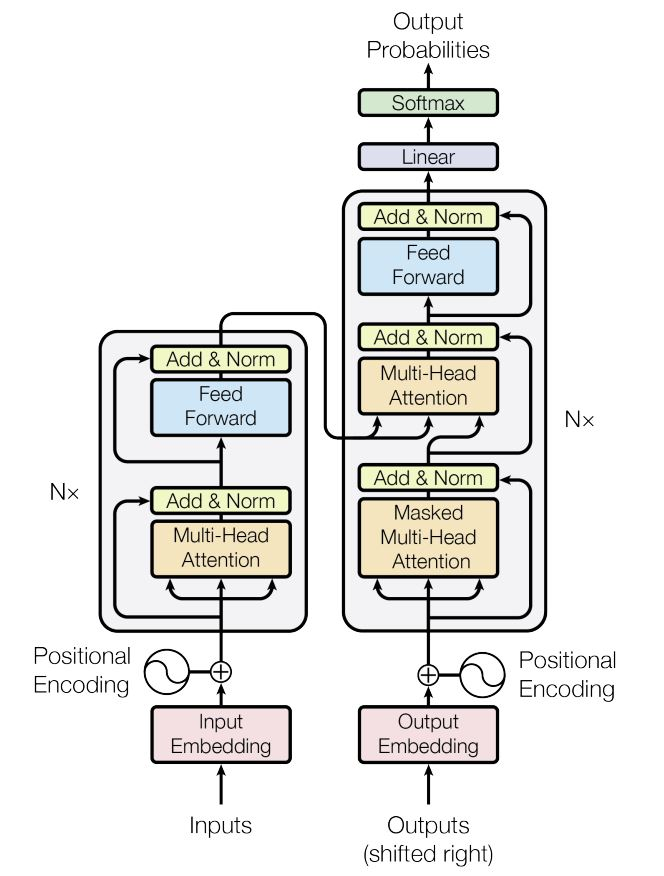
\includegraphics[width=0.5\textwidth]{chapters/images/Transformer/Architecture.JPG}
    \caption{Model Architecture\cite{vaswani2017attention}}
    \label{fig:Model_Architecture}
\end{figure}

\subsection{Overview of transformer model architecture}

The transformer architecture is made of encoder and decoder as shown left and right respectively in \Cref{fig:Model_Architecture}. A Comprehensive introduction of components and its functionality is described in paragraphs below.

\subsubsection{Input Embedding}
It is the first component in both encoder and decoder. This layer takes input sequence and convert it into vectors that is also known as continuous representation. It maps each word  and provide numerical value to each word.

\subsubsection{Positional encoding}
In this step, the positional information is being injected to the vector representation derived from input embedding layer. Transformer uses wave function to give positional information to input embedding by creating vectors for odd and even positions using cosine and sine function respectively (\Cref{eq:Wave_functions}).

\begin{equation}
    \label{eq:Wave_functions}
    PE_{(pos, 2i)} = \sin{\left(\frac{pos}{10000^\frac{2i}{d_{model}}}\right)}
\end{equation}
\[PE_{(pos, 2i+1)} = \cos{\left(\frac{pos}{10000^\frac{2i}{d_{model}}}\right)} \]

\subsubsection{Encoder Layer}


\begin{figure}[ht]
    \centering
    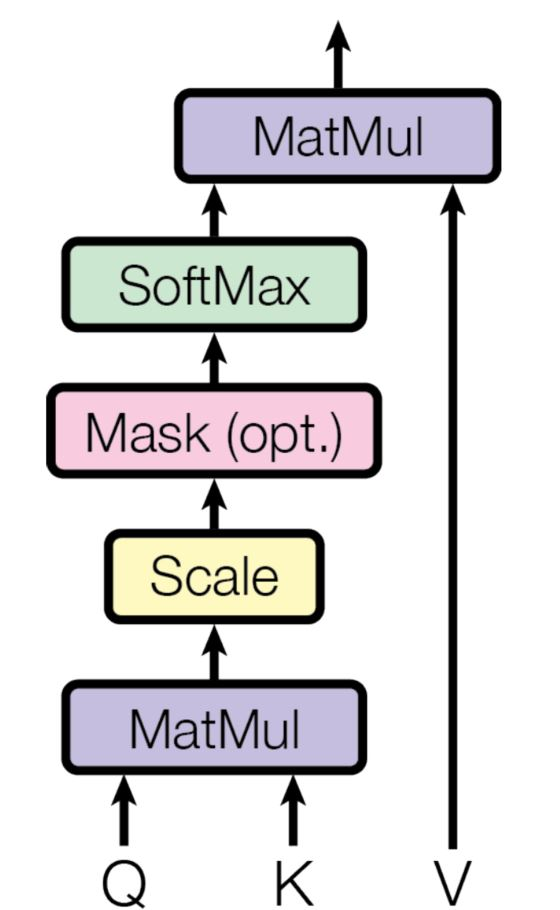
\includegraphics[width=0.25\textwidth]{chapters/images/Transformer/Inside_Attention.JPG}
    \caption{Scaled Dot-product Attention \cite{vaswani2017attention}}
    \label{fig:Scaled_Dot-product_Attention}
\end{figure}

The encoder layer is made of two sub-layer, multi-headed attention followed by fully connected feed forward network (\Cref{fig:Model_Architecture}). Multi-headed attention layer uses self-attention that allows the model to associate each word to other words in input embedding. To achieve self-attention, input embedding are passed through three linear layers to obtain query, key and value vectors represented as Q, K and V in \Cref{fig:Scaled_Dot-product_Attention}. As an example, if a word or sentence we used to search something in Google search are queries, the websites that Google search will provide are keys and the content of the websites are Values. Matrix multiplication step uses these queries and keys to obtain score matrix. The score matrix shows how much attention a word should keep into other words. These scores are then divided using square root of the dimension of queries and keys to scale it down to obtain stable gradients during values multiplication. After that the softmax is being taken to get the attention weights or attention filter. Softmax is a function that takes each vectors from scale matrix, normalizes it and gives the probabilistic distribution so that each component in matrix will be in interval of (0,1). By doing so, the higher score will be heightened and lower scores will be depressed providing model confident values to attend words accordingly. Later on, these attention weights are multiplied with value vectors (\Cref{eq:Attention}). The higher softmax scores will keep the word that is more important and lower softmax scores will soften the words that are irrelevant. After that query, key and value vectors are splited into N vectors and applied to self-attention individually therefore known as multi-headed attention computation where each self-attention process is called head. Each head will produce output vector which will be concatenated into a single vector. This way each head will learn something different than other layers. 
\begin{equation}
    Attention(Q,K,V) = softmax\left(\frac{QK^T}{\sqrt{d_k}}\right)V
    \label{eq:Attention}
\end{equation}


\begin{figure}[hb]
    \centering
    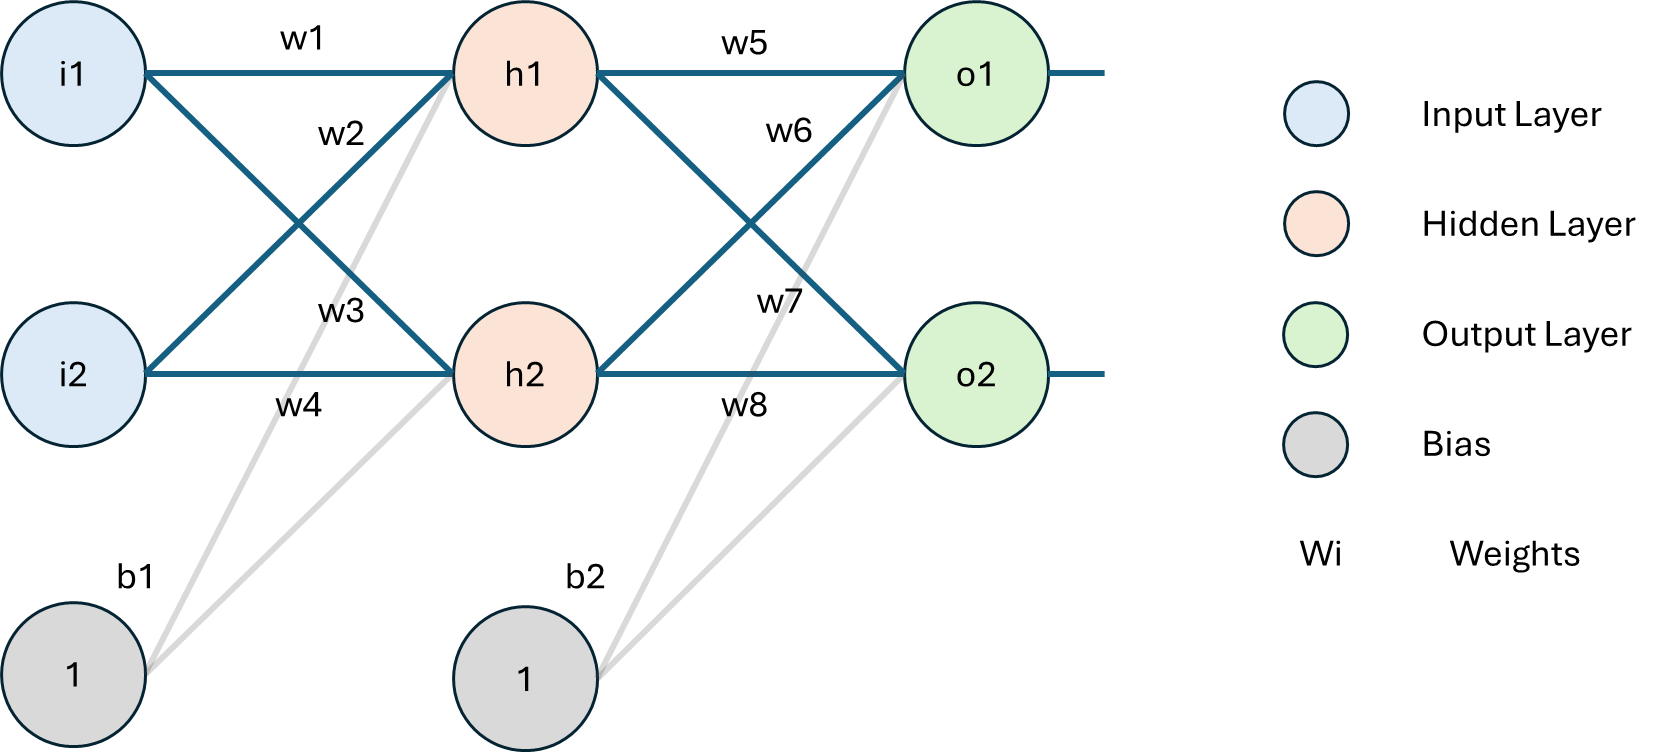
\includegraphics[width=0.7\textwidth]{chapters/images/Transformer/neuralnet.png}
    \caption{Diagram of neural network with different layers}
    \label{fig:neuralnet}
\end{figure}

The block "Feed Forward" in \Cref{fig:Model_Architecture} refers to the term multi-layered networks of neurons and information in these layers flows into one direction hence is pronounce feedforward. The network is made of Input Layer, Hidden Layer and Output Layer. In \Cref{fig:neuralnet} a simple neural network with two input, two hidden and output neurons has been shown. The goal is to find a weights for hidden layer and output layer in a way that Network takes the input and compute with these weights assigned to hidden and output neurons and try to predict the desired or nearest output. In initial phase, these weights assigned to hidden layer and output layer can be random or the attention derived from attention mechanism. In the process Forward Pass, the input values are passed to hidden layers. Total input value will be derived at each hidden node and then being squash using activation function like ReLU \cite{ReLU}, tanh \cite{tanh}. These activation functions help neural network to be non-linear allowing neural networks to expand complex representations and functions that is not possible with a linear regression model. Weights shows the strength of the connection between layers and biases make sure that if the input value is 0 than in activation function the output is not 0. The process is repeated for the output layer using the output of hidden layer as a inputs. Once we receive the outputs at output layers based on initial weights, the total error is being calculated based on targeted values. Once we have the total error of the network the process "Backwards pass" starts in which algorithm like "backpropagation" is used to calculate the gradient according to the total error using "Chain rule" for each node. Sometimes the learning rate is being used to multiply this gradient with the learning rate and then subtracted from the initial weights resulting in new weights. Then the process is repeating but this time with the new weights and is being repeated until the network provide outputs near to the targeted value. 

All these operation serves the prime purpose of encoding the input into a continuous representation with attentions so that decoder can focus on suitable word in the input while decoding. One can stack the encoder layers to encode the inputs in order to further encode the information. By doing so each layer can learn different attention representation that boosts the predictive power of the transformer network. 

\subsubsection{Decoder layer}
The decoder is responsible to generate the text sequences from the output vectors from encoder. It has similar sub layers as the encoder one multi-headed attention layers and feed-forward layer. The decoder is auto regressive that uses the previous outputs as inputs and uses encoder outputs that includes the attention information from input.

The input goes to embedding layers to obtain positional embedding. After that, these position aware vectors goes through multi-headed attention layer to generate the scores which later will be used as a decoder input. The next multi-headed attention layers works slightly different. Due to the fact that decoders are autoregressive and omit the sequence word-by-word, a condition is applied where it uses the positions to insure that prediction for position $i$ can only depend on known outputs at positions less than $i$. This process also known as mask where all the position greater than $i$ will be assigned as negative infinity so that when the softmax will be performed, there will be zero attention scores for future tokens. The output of the first multi-headed attention layer is mask output vector which will be used as a values for second multi-headed attention and the encoder output will be taken as keys and queries. The output second multi-hesded attention layer goes through to feed forward where the output will go through linear layer that act as a classifier, Here, the softmax layer will provide probaility score to each class between 1 and 0. The one with highest probability score will be taken as predicted word. The decoder can also be stacked N times that takes inputs from the encoder and the layers before it, which helps model to focus and extract on different combinations of attention, attention heads resulting in a boost in predictive power.
% \begin{equation}
%     Attention(Q,K,V) = softmax\left(\frac{QK^T}{\sqrt{d_k}}\right)V
%     \label{eq:Attention}
% \end{equation}





% Most used structure for transforming sequence is encoder-decoder. Where encoder uses input sequence as $(x_1, x_2, ..., x_n)$ and convert it into continuous representations (numerical representation) z = $(z_1, z_2, ..., z_n)$. The decoder takes this given z and generates an output sequence $(y_1, y_2, ..., y_n)$ using one element at a time. Model is auto-regressive at each steps \cite{graves2013generating}, that uses the former result as a additional input in order to generate the next result. The Transformer uses this overall architectures in addition with self-attention with connected encoder and decoder (left and right respectively in Figure \ref{fig:Model_Architecture}).






% The encoder contains 6 identical layers where each layers contains two sub-layers. The first layer is a multi-head self-attention mechanism and second layer is feed-forward network. Each sub-layers of this layers is using residual connections \cite{he2016deep} (please refer to \ref{residual_connection}) which will be normalized using normalization layer \cite{ba2016layer} resulting LayerNorm(x+Sublayer(x)). Sublayer(x) is the function implemented by sub-layer itself. All these residual connections, sub-layers and embedding layers produces outputs of 512 dimension. Decoder also contains 6 layers with its sub-layers. Decoder takes the output of Encoder layer and performs self-attention, uses residual connections with normalization. In Decoder, the self-attention sub-layer is modified where it uses the positions to insure that prediction for position $i$ can only depend on known outputs at positions less than $i$.

% \subsection{residual connections \label{residual_connection}}
% \cite{Residual_connection}




% \subsection{Attention Mechanism\label{attention}}
% Transformer became prime component in natural language processing due to its ability to process long text and generate results and text while maintaining the context. Figure \ref{fig:Scaled_Dot-product_Attention} shows different components of "Multi-Head Attention" layer in Figure \ref{fig:Model_Architecture}. Where Q, K and V represents Query, Key and Value respectively. As an example, Query can be a word or sentence we used to search something in google search, Keys can be the websites that google search will provide which is similar to query and Value can be the content of the websites. The similarity between Query and Key are computed using \textbf{Cosine Similarity} ranging from +1 to -1. In Figure \ref{fig:Model_Architecture} in both encoder and decoder, Inputs are simply embedding of words, a fixed-length vectors. Machine translation algorithm like RNN, CNN and LSTM takes one input embedding at a time in a sequential manner, while Transformers take all embedding as a whole, Hence the \textbf{Positional Encoding} has been introduced in order to add information of word order to the vectors. In paper \cite{vaswani2017attention}, positional encoding has been achieved using wave frequencies \ref{eq:Wave_functions} to provide each word a unique position embedding.





% Once we have position aware matrices of Query, Key and Value, the steps mentioned in Figure \ref{fig:Scaled_Dot-product_Attention} will be performed in which in the step "MatMul" the dot product of matrices Q and K is being taken in order to find similarity also known as providing score. In step "Scale" we divide the score in order to scale, \(\sqrt{d_k}\) is used in paper \cite{vaswani2017attention} where \(d_k\) represents dimension of keys. In the next step the Softmax is being taken in order to squash the results between 0 and 1 at this stage the resultant matrix is so called \textbf{Attention Filter}. Finally, multiplying this Attention Filter to Value matrix gives us the \textbf{Attention} \ref{eq:Attention}.

% \begin{equation}
%     Attention(Q,K,V) = softmax\left(\frac{QK^T}{\sqrt{d_k}}\right)V
%     \label{eq:Attention}
% \end{equation}

% \subsection{Feed Forward\label{feed forward}}
% \begin{figure}[ht]
%     \centering
%     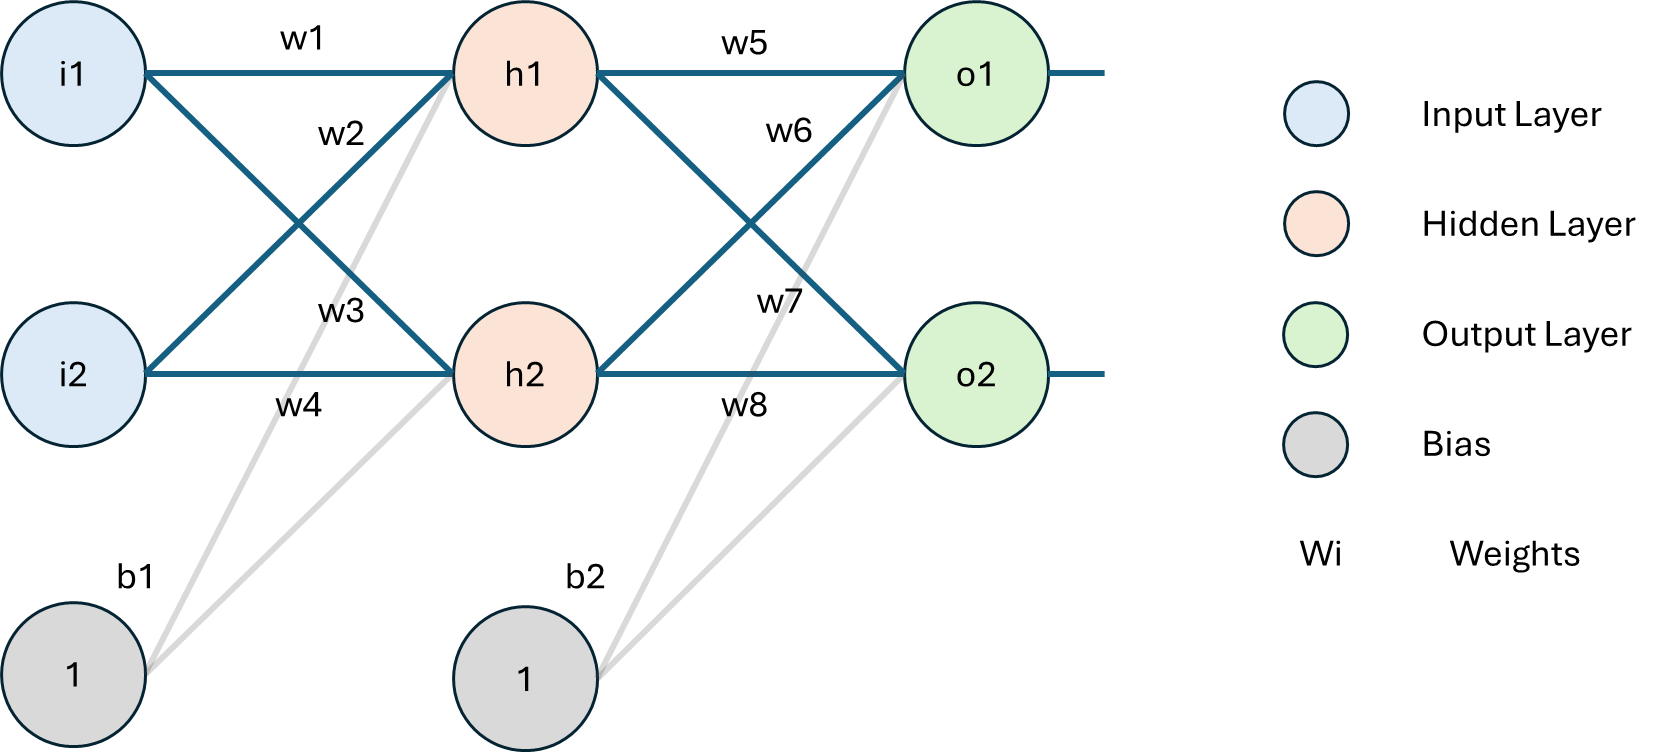
\includegraphics[width=0.7\textwidth]{chapters/images/Transformer/neuralnet.png}
%     \caption{Diagram of neural network with different layers}
%     \label{fig:neuralnet}
% \end{figure}

% The block "Feed Forward" in figure \ref{fig:Model_Architecture} refers to the term multi-layered networks of neurons and information in these layers flows into one direction hence is pronounce "feedforward". The network is made of Input Layer, Hidden Layer and Output Layer. In Figure \ref{fig:neuralnet} a simple neural network with two input, two hidden and output neurons has been shown. The goal is to find a weights for hidden layer and output layer in a way that Network takes the input and compute with these weights assigned to hidden and output neurons and try to predict the desired or nearest output. In initial phase, these weights assigned to hidden layer and output layer can be random or the attention derived from attention mechanism. In the process Forward Pass, the input values are passed to hidden layers. Total input value will be derived at each hidden node and then being squash using activation function like ReLU \cite{ReLU}, tanh \cite{tanh}, Softmax and so on. These activation functions help neural network to be non-linear. Weights shows the strength of the connection between layers and biases make sure that if the input value is 0 than in activation function the output is not 0. The process is repeated for the output layer using the output of hidden layer as a inputs. Once we receive the outputs at output layers based on initial weights, the Total Error is being calculated based on targeted values. Once we have the total error of the network the process "Backwards pass" starts in which algorithm like "backpropagation" is used to calculate the gradient according to the total error using "Chain rule" for each node. Sometimes the learning rate is being used to multiply this gradient with the learning rate and then subtracted from the initial weights resulting in new weights. Then the process is repeating but this time with the new weights and is being repeated until the network provide outputs near to targeted value. 
